\subsection{Основные понятия.}

\deff{def:} $f: R^n  \rightarrow \R$ - $\forall x \in \R^n f(x)= \sum\limits_{i=1}^n \sum\limits_{j=1}^n a_{ij}x_ix_j$ - \deff{квадратичная форма}, причем $a_{ij} = a_{ji}$

$f(x) = x^T A x$ - \deff{матричная форма записи}.

$f(x) = 2 \sum\limits_{1 \leq i < j \leq n}a_{ij} x_i x_j + \sum\limits_{i=1}^n a_{ii}x_i^2$

\textbf{Замечание:} $\alpha: V \times V \rightarrow \R$, $\dim V = N, \alpha \in T(2,0)$, билинейная форма, а также симметричная форма. И тогда:
$$f(x) = \alpha(x,x)$$

\deff{def:} $\rg f = \rg A$.

\deff{def:} Говорят что к квадратичной форму $f$ \deff{применено лин. преобразование} $Q$ (невырожденное), если $x = Qy$:
$$g(y) = f(Qy) = (Qy)^T A Qy =  y^T (Q^TAQ)y$$
$g$ квадратичная форма с матрицей $B = Q^TAQ$.

\textbf{Замечание:} $\rg f =\rg B = \rg \, g$

\textbf{Замечание:} Иногда мы будем думать о матрице $Q$ таким образом: $Q$ невырожденная $\Rightarrow Q$, матрица перехода из $T_{\text{кан}\rightarrow q}, x = Qy$, где $x$ старые координаты, а $y$ новые.

возможно стоит переформулировать

\deff{def:} Говорят, что квадратичная форма $f$ приведена к \deff{канонич.} виду линейным невырожденным преобразованием $Q$, если $B  = diag(b_{11},\ldots, b_{nn})$.
$$f(x) = g(y) = b_{11}y_1^2 + \ldots + b_{nn}y_n^2$$
$\sigma^+(f)$ - количество $b_{ii}>0$ --- \deff{положительный индекс инерции}.

$\sigma^-(f)$ - количество $b_{ii}<0$ --- \deff{отрицательный индекс инерции}.

$\sigma^0(f)$ - количество $b_{ii}=0$

$\sigma = (\sigma^+, \sigma^-, \sigma^0)$ называется \deff{сигнатурой} квадратичной формы $f$.

\textbf{Замечание:} Периодами в литературе встречается $\sigma = \sigma^+ - \sigma^-$.

Основная задача теории кв. форм: Существует ли такая $Q$ невырожденная и если существует, то как ее найти.

\deff{def:} Канонический вид формы называется \deff{нормальным}, если $\forall i : b_{ii} = \pm 1$ или 0.

\textbf{Замечание:} Любую квадратичную форму из канонического вида всегда можно привести к нормальному. И делается это тривиально.

\newpage

\subsection{Основные методы приведения квадратичной формы к каноническому виду.}

\textbf{Задача:} 

$f(x) = x^T Ax,A = A^T$. Существует ли $Q$ невырожденная, что $x = Qy$, $f(x) = g(y) = y^TBy$ и $B = Q^TAQ = diag(b_{11},\ldots, b_{nn})$


\deff{I. Ортогональное преобразование.}

См. следствие к теореме о каноническом виде матрицы самосопряженного оператора:

$A = A^T, \exists T$ ортог. $T^T  A T = \Lambda = diag(\lambda_1,\ldots,\lambda_n)$ и это $Q$ и есть $T$.

$Q = (q_1,\ldots,q_n), V_\lambda \perp V_\mu$

$f(x) = \lambda_1 y_1^2 + \ldots + \lambda_n y_n^2$

\textbf{Замечание:} матрица $Q$ не нужна для вычисления канонического вид. При этом, чтобы найти $Q$ нам нужно найти собственные подпространства и получить ортогональный базис из собственных векторов.

\deff{II. Метод Лагранжа.}

$f(x) = 2 \sum\limits_{1 \leq i <j \leq n}a_{ij}x_i x_j + \sum\limits_{i=1}^n a_{ii}x_i^2$

Метод:
\begin{enumerate}
    \item Если все $a_{ii}=0$, тогда существует $a_{ij}\neq 0$, $x=Qy$. Пусть $Q$ будет выполнять:
    $$\begin{cases}
        x_i = y_i + y_j \\
        x_j  = y_i - y_j\\
        x_k = y_k, k\neq i, k \neq j
    \end{cases}$$
    Очевидно $Q$ невырожденно.
    \item $\exists a_{ii}\neq 0$. Выпишу все такие элементы:
    $$a_{ii}x_i^2 + 2\sum\limits_{i \neq j}a_{ij}x_ix_j = \cfrac{1}{a_{ii}}(a_{ii}^2 x_i^2 + 2\sum\limits_{j\neq i} a_{ij} a_{ii}x_i x_j) = \cfrac{1}{a_{ii}} \left(\sum\limits_{j=1}^n a_{ij} x_j\right)^2 - \cfrac{1}{a_{ii}}\sum\limits_{j \neq i}a_{ij} x_j^2 -  \cfrac{2}{a_{ii}}\sum\limits_{i\neq j, k \neq i} a_{ij}a_{ik}x_j x_k$$
    Давайте сделаем замену $Q$:
    $\begin{cases}
    y_i = \sum\limits_{j=1}^n a_{ij}x_j\\
    y_k = x_k, k \neq i
    \end{cases}$. Она будет иметь вид:
    $$Q^{-1}= \begin{pmatrix}
        1 & & & & &  & \\
         & \ddots& & & &  & \\
         & & 1& & &  & \\
         a_{i1}&\ldots &\ldots &a_{ii} &\ldots &\ldots  &a_{in} \\
         & & & & 1&  & \\
          & & & & &  \ddots& \\
           & & & & &  &1 \\
    \end{pmatrix}$$
    Откуда очевидно невырожденная, а то есть и сама $Q$ невырожденная.

    Заметим, что после такого преобразования у нас пропадают все элементы $a_{ij}$ с $i \neq j$.

    \item $f(x) = g(y) = \cfrac{1}{a_{ii}}y_i^2 + t(y_1,\ldots, \hat{y_i},\ldots, y_n)$ --- функция от $n-1$ переменной. Повторить пункт 1 для функции $t$.
\end{enumerate}

\textbf{Замечание:} метод Лагранжа применим для любых квадратичных форм, но, в отличие от ортог. преобразования, не позволяет сразу записать канонический вид.


\deff{III. Метод Якоби (LDU разложение)}

Хотим получить $Q$ - унитреугольная верхняя. 

$\Delta_k \neq 0 , k = 1,\ldots, n-1; A= A^T$, откуда можно применить теорему об $LDU$ разложении, которая гласит, что $\exists! L, \exists! D, \exists! U$, что $A = LDU$. Из следствия теоремы получаем, что для самосопряженных операторов: $L^T=L^* = U$.

Откуда если обозначить за $Q = (L^{-1})^T$, то $B = Q^T AQ$

При этом  $B = diag(d_1,\ldots,d_n)$, где $d_{i+1} = \cfrac{\Delta_{i+1}}{\Delta_i}$

Откуда, построив $LDU$ разложение, мы можем быстро найти нужную нам $Q$.


\thmm{Теорема: (метод Якоби)}

$\forall k = 1 \ldots n-1: \Delta_k\neq 0 : f(x) = x^TAx: A = A^T$

Хотим показать, что существует и единственна унитреугольная верх:
$$Q: B = Q^T AQ = diag(\Delta_1, \cfrac{\Delta_2}{\Delta_1},\ldots , \cfrac{\Delta_n}{\Delta_{n-1}})$$
Введем вот такие обозначения:
\begin{center}
   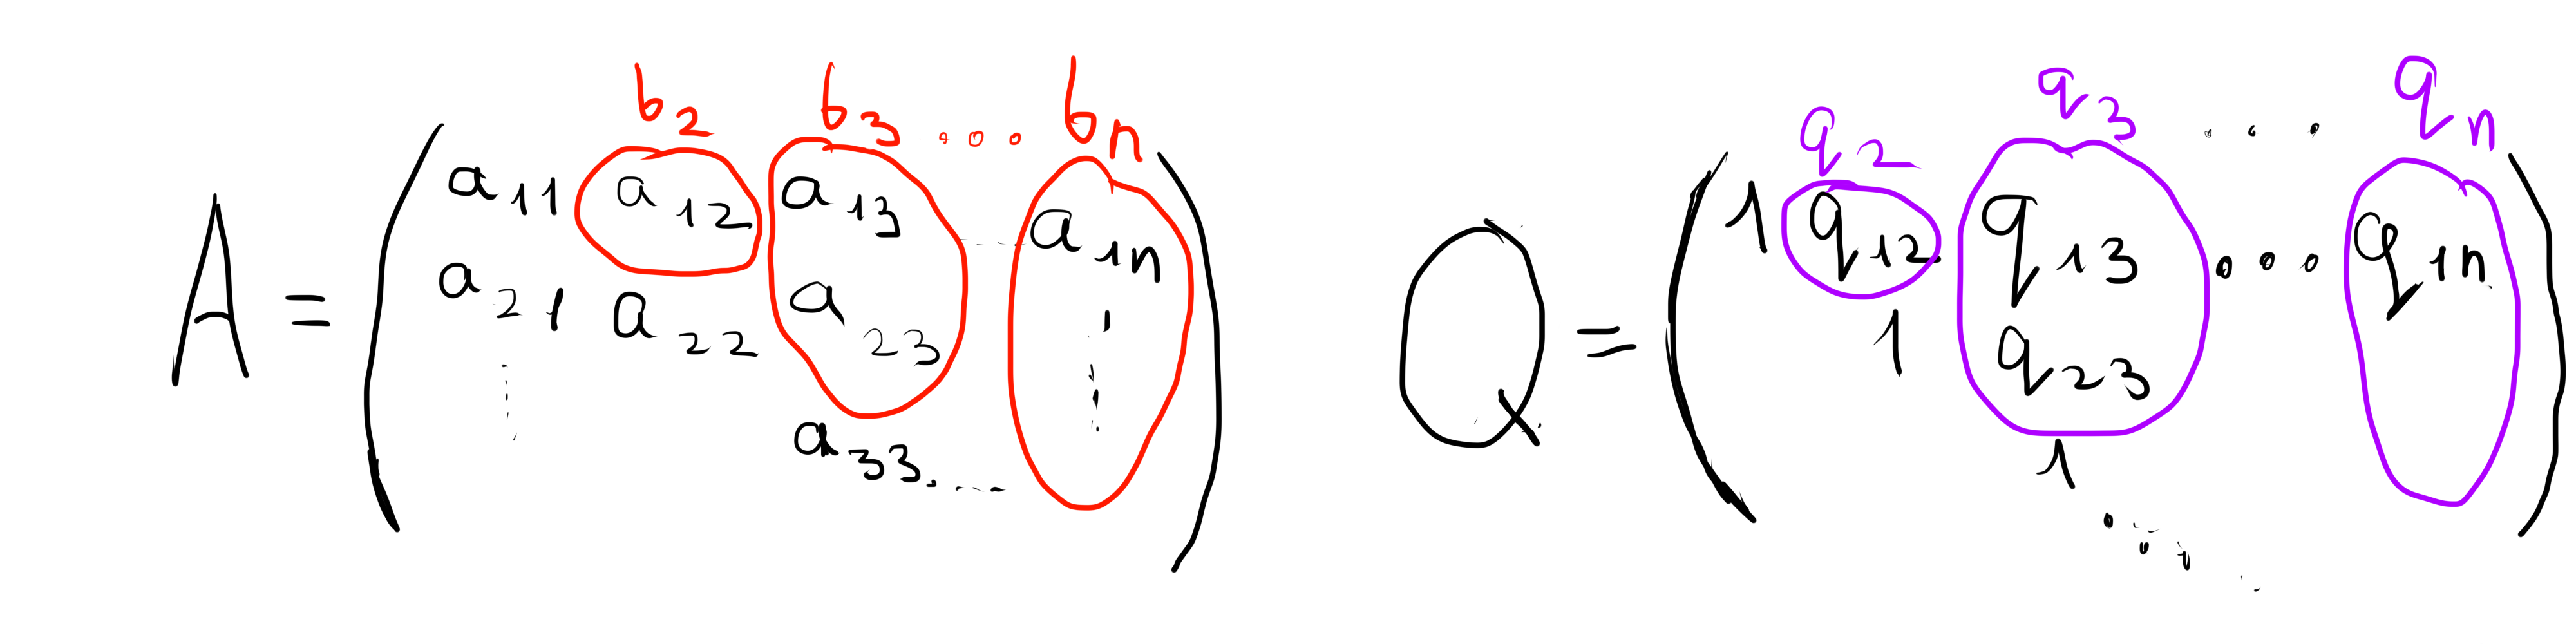
\includegraphics[width = 17cm]{assets/11_2-forms.png}
\end{center}
И будет выполнено: $A_k q_{k+1} = -b_{k+1}$ для всех $k= 1\ldots n-1$, где $A_k$ - угловая матрица размера $k$, причем для каждого уравнения будет единственное решение так как $\Delta_k = \det A_k \neq 0$.

\textbf{Доказательство:}

\textbf{Замечание:} Единственность следует из $LDU$ разложения, нам нужно доказать только формулу

Воспользуемся методом математической индукции.

\uline{База:} $n=2$ оставим читателю.

\uline{Индукционное предположение:} Пусть формула верна для $k$. Проверим, что верна для $k+1$.

Пусть $Q_{k+1} = \begin{pmatrix}[c|c] 
    Q_k& q_{k+1}\\
    \hline  0 & 1
\end{pmatrix}$. где $q_{k+1}$ это решение нашей системы. Хотим понять чему равно
$Q_{k+1}^T A_{k+1}Q_{k+1}$. Распишем:
$$Q_{k+1}^T A_{k+1}Q_{k+1} =\begin{pmatrix}[c|c] 
    Q_k^T& 0\\
    \hline  q_{k+1}^T & 1
\end{pmatrix} \begin{pmatrix}[c|c] 
    A_k& b_{k+1}\\
    \hline  b_{k+1}^T & a_{k+1 k+1}
\end{pmatrix} \begin{pmatrix}[c|c] 
    Q_k& q_{k+1}\\
    \hline  0 & 1
\end{pmatrix}  =$$ $$=\begin{pmatrix}[c|c] 
    Q_k^T& 0\\
    \hline  q_{k+1}^T & 1
\end{pmatrix}  \begin{pmatrix}[c|c] 
    A_k Q_k& A_k q_{k+1} + b_{k+1} = 0\\
    \hline  b_{k+1}^T Q_k & b_{k+1}^Tq_{k+1} + a_{k+1 k+1}
\end{pmatrix} =$$
$$= \begin{pmatrix}[c|c] 
    Q_k^TA_k Q_k& 0\\
    \hline  q_{k+1}^TA_kQ_k + b_{k+1}^T Q_k& b_{k+1}^Tq_{k+1} + a_{k+1 k+1}
\end{pmatrix} =$$
Заменим $A_k = A_k^T$ и получим:
$$=\begin{pmatrix}[c|c] 
    Q_k^TA_k Q_k& 0\\
    \hline  (q_{k+1}^TA^T_k + b_{k+1}^T) Q_k& b_{k+1}^Tq_{k+1} + a_{k+1 k+1}
\end{pmatrix} = $$
Используя то, что $q_{k+1}^TA^T_k + b_{k+1}^T = A_kq_{k+1} + b_{k+1} = 0$ и и.п. получаю:
$$=\begin{pmatrix}[c|c] 
     D_k& 0\\
    \hline  0 & d_{k+1}
\end{pmatrix} $$
\hfill Q.E.D.
\newpage 

\subsection{Закон инерции кв-формы. Критерий Сильвестра.}

\thmm{Теорема (закон инерции кв. формы)}

Каким бы линейным невырожденным преобразованием квадратичная форма не была приведена к каноническому виду, сигнатура полученной формы будет одинаковой.

$f(x)$ - квадратичная форма. $f(x) = x^TAx, A= AT$, $x= Q_1 y, x = Q_2y, Q_1,Q_2$ невырожденна. 

$f(x) = g(y) = t(z) \Rightarrow \sigma(g) = \sigma(t)$.

\textbf{Доказательство:}

Будем доказывать от противного: Пусть $p<s$:
$$g(y) = \lambda_1 y_1^2 + \ldots + \lambda_p y_p^2 - \lambda_{p+1} y_{p+1}^2 - \ldots - \lambda_r y_r^2$$
$$f(y) = \mu_1 y_1^2 + \ldots + \mu_s y_s^2 - \lambda_{s+1} y_{s+1}^2 - \ldots - \lambda_r y_r^2$$
$$B = Q_1^TAQ_1 = diag(\lambda_1,\ldots,\lambda_p, -\lambda_{p+1},\ldots, -\lambda_r, 0 ,\ldots,0)$$
$$C = Q_2^TAQ_2 = diag(\mu_1,\ldots,\mu_s, -\mu_{s+1},\ldots, -\mu_r, 0 ,\ldots,0)$$ 

$r = \rg(f) = \rg (g) = \rg(t)$

Посмотрим на парочку уравнений:

$y = Q^{-1}_1x, z = Q_2^{-1}x$

Заметим, что $p+n-s < n$.

Возьмем первые $p$ уравнений из $Q^{-1}_1$ и последние $n-s$ из $Q_2^{-1}$. Получим СЛОУ с новой матрицей $\tilde{Q}$. Заметим, что количество строк в ней меньше $n$ а значит есть нетривиальное решение $x_0 \neq \zero$. Тогда для этого $x_0$ будет выполнено:

$y_0 = Q^{-1}_1x_0 = \begin{pmatrix}
    0\\
    \vdots\\
    *
\end{pmatrix}$ (первые $p$ нули), \quad 
$z_0 = Q^{-1}_2x_0 = \begin{pmatrix}
    p\\
    \vdots\\
    0
\end{pmatrix}$ (последние $n-s$ нули). 

При этом $f(x_0) = g(y_0) = -\lambda_{p+1} \ldots = t(z_0)=\mu_1 \ldots $. 

С одной стороны я получаю только отрицательные $\lambda$ с соотв $y_i^2$, с другой стороны я получаю только положительные $\mu$ с соотв. $z_j^2$. Тогда:
 $-\lambda_{p+1} \ldots = \mu_1 \ldots $, но я знаю, что хотя бы с одной стороны есть ненулевая координата (из новорожденности ). Откуда противоречие.

\hfill Q.E.D.

\textbf{Замечание:} после теоремы можно корректно ввести понятие $\sigma(f)=\sigma(g)= \sigma(t)$ не зависит от $Q$.

\deff{def:} Знакопределенность кв. ф.

\begin{enumerate}
    \item $f > 0 \Leftrightarrow \forall x \in \R^n: f(x)>0 \Leftrightarrow A >0$
    \item $f<0 \Leftrightarrow A<0$
    и аналогично с другими определенностями, которые у нас уже были
\end{enumerate}

\thmm{Теорема (Критерий Сильвестра)}

$f(x)  = x^T Ax , A = A^T, \Delta_k \neq 0 , k = 1\ldots n$. Тогда:
$$f >0 \Leftrightarrow \Delta_k > 0, k = 1, \ldots, n$$
$$f <0 \Leftrightarrow (-1)^k \Delta_k >0, k = 1\ldots n$$
\textbf{Доказательство:}

$f>0$ по методу Якоби $x = Qy \exists !$ унитреугольная вертикальная 

я не понял

\hfill Q.E.D.

\pagebreak


\subsection{Приведение ПВП к канон. виду.}

см фото, добавится ближе к экзамену